\chapter{Desarrollo de la Solución}
Dentro de esta sección se expone con precisión el procedimiento descrito previamente en la sección anterior, correspondiente a cada acción incluida en la metodología implementada, junto con los entregables previstos.

\section{Adquisición de los Datos}

\textbf{Actividad 1: Identificación de la data que contengan imágenes de rostros con características morfológicas faciales de proporciones similares}
 
Con el objetivo de entrenar un modelo de segmentación enfocado en características morfológicas faciales como arrugas y manchas, se llevó a cabo una exhaustiva búsqueda de bases de datos públicas en repositorios especializados. Se priorizó la recolección de conjuntos de datos que incluyeran imágenes faciales en alta resolución, variedad de edades, géneros y tonos de piel, así como condiciones de iluminación lo suficientemente controladas como para facilitar la segmentación de detalles faciales sutiles.

Durante este proceso, se identificaron diversos repositorios en plataformas como GitHub que ofrecían acceso a bases de datos con más de 200,000 imágenes faciales. Entre los conjuntos más destacados se encuentran versiones extendidas de datasets como CelebA, FFHQ (Flickr-Faces-HQ), y otros compendios curados por la comunidad investigadora, que contienen imágenes faciales etiquetadas o anotadas para tareas de reconocimiento y análisis facial.

Sin embargo, debido al enfoque específico de esta investigación la segmentación de características morfológicas finas como arrugas y manchas fue necesario realizar una selección cuidadosa de las imágenes más adecuadas. Para ello, se aplicaron criterios de claridad visual, resolución suficiente y visibilidad explícita de las deformaciones morfológicas faciales. Como resultado de este filtrado, se seleccionó un subconjunto compuesto por 5,000 imágenes faciales que cumplían con los siguientes criterios:

\begin{itemize}
    \item Alta calidad visual.   
    \item Visibilidad clara de texturas de la piel.
    \item Presencia evidente de arrugas y manchas.
    \item Proporciones faciales dentro de un rango estándar para facilitar el modelado.
\end{itemize} 

Este conjunto reducido pero representativo,lo podemos ver en la Figura \ref{4:fig1}, constituye la base de entrenamiento y validación del modelo propuesto. La selección manual de estos datos buscó optimizar el desempeño del modelo, al exponerlo exclusivamente a ejemplos que contienen información útil para aprender patrones asociados a las características morfológicas de interés.

\begin{figure}[h]
	\begin{center}
		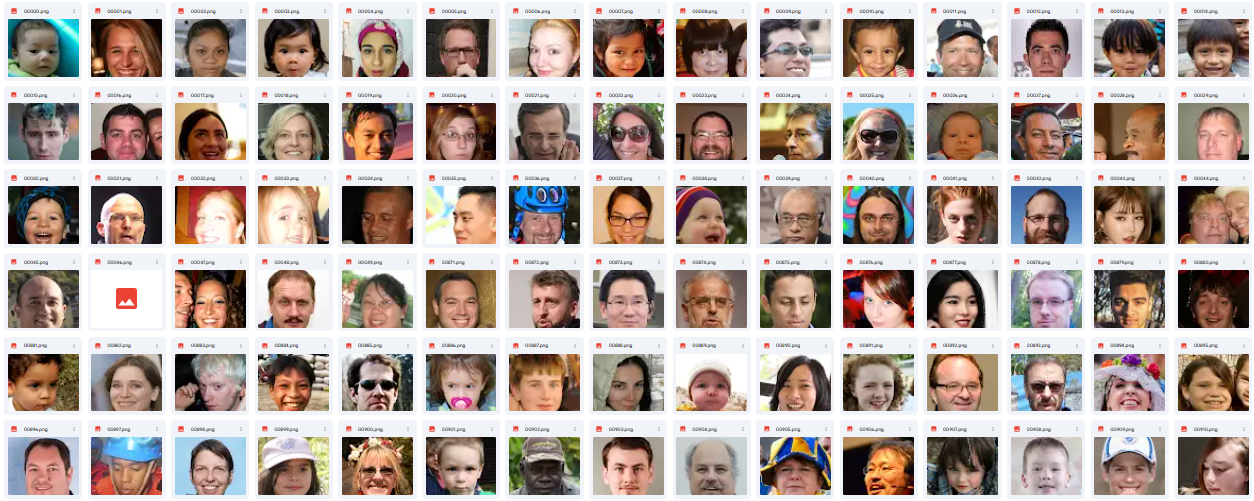
\includegraphics[width=0.75\textwidth]{4/figures/data.png}
		\caption[Dataset recolectado de repositorios]{Dataset recolectado de repositorios.\\
		Fuente: Elaboración propia}
		\label{4:fig1}
	\end{center}
\end{figure}

\section{Preprocesamiento de los Datos}

\textbf{Actividad 1: Filtración de imágenes faciales con características morfológicas}

Una vez recopilado el subconjunto de 5,000 imágenes faciales con características morfológicas visibles, se procedió a una etapa de filtración adicional orientada a reforzar la consistencia y la relevancia de los datos para la tarea de segmentación. Esta filtración se enfocó en garantizar que todas las imágenes seleccionadas contuvieran arrugas y manchas claramente identificables, descartando aquellas que, pese a su calidad visual, no presentaban estas características de manera explícita.

El proceso se realizó mediante una inspección semiautomática, apoyada en técnicas básicas de detección de texturas y realce de bordes para facilitar la identificación visual de las zonas con deformaciones. Como resultado, se aseguraron condiciones homogéneas entre las imágenes del dataset final, lo que permitió una base sólida para la generación de máscaras de segmentación precisas.

\textbf{Actividad 2: Representación y normalización de las imágenes faciales}

Con el conjunto de imágenes definitivo, se ejecutó un proceso de preprocesamiento estandarizado con dos objetivos principales: uniformar las dimensiones espaciales de las imágenes y generar las máscaras binarias asociadas a las regiones con deformaciones morfológicas.

En primer lugar, todas las imágenes fueron redimensionadas a una resolución uniforme de 1024x1024 píxeles, preservando la relación de aspecto y aplicando interpolación bilineal para mantener la calidad visual. Esta estandarización es fundamental para asegurar la compatibilidad estructural con las redes neuronales convolucionales utilizadas en etapas posteriores, y facilita la aplicación de operaciones convolucionales sobre áreas homogéneas.

En segundo lugar, se generaron máscaras binarias (en blanco y negro) correspondientes a cada imagen. Estas máscaras representan las regiones específicas del rostro que contienen arrugas, manchas u otras alteraciones morfológicas, codificadas de la siguiente manera:

\begin{itemize}
    \item Blanco (valor 1): Regiones con características morfológicas relevantes (objetivo de segmentación).   
    \item Negro (valor 0): Regiones sin interés morfológico.
\end{itemize} 

Las máscaras, como se ve en la Figura \ref{4:fig2}, fueron elaboradas a partir de una combinación de anotación semiautomática y herramientas de realce de texturas, contrastes y gradientes, con verificación manual en una muestra aleatoria para asegurar su validez.

\begin{figure}[h]
	\begin{center}
		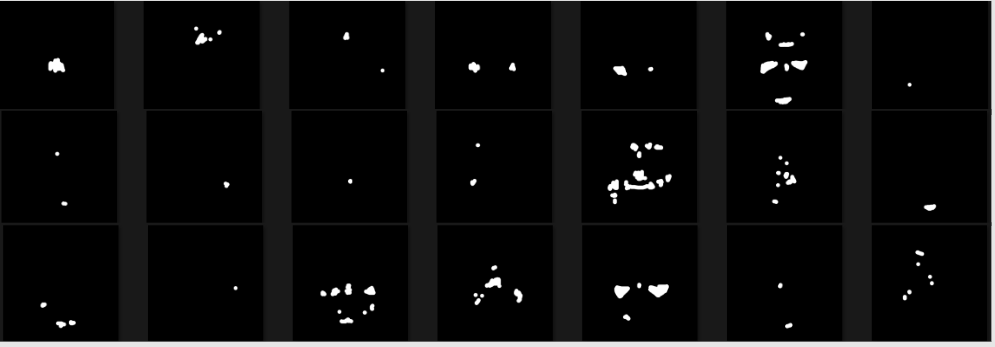
\includegraphics[width=0.75\textwidth]{4/figures/mascaras.png}
		\caption[Máscaras binarias generadas]{Máscaras binarias generadas.\\
		Fuente: Elaboración propia}
		\label{4:fig2}
	\end{center}
\end{figure}

Este proceso de representación y normalización, como se ve en el diagrama final de Preprocesamiento en la Figura \ref{4:fig3}, permitió convertir los datos originales en pares de entrada (imagen facial) y salida (máscara de segmentación), aptos para el entrenamiento supervisado del modelo de segmentación basado en redes neuronales convolucionales.

\begin{figure}[h]
	\begin{center}
		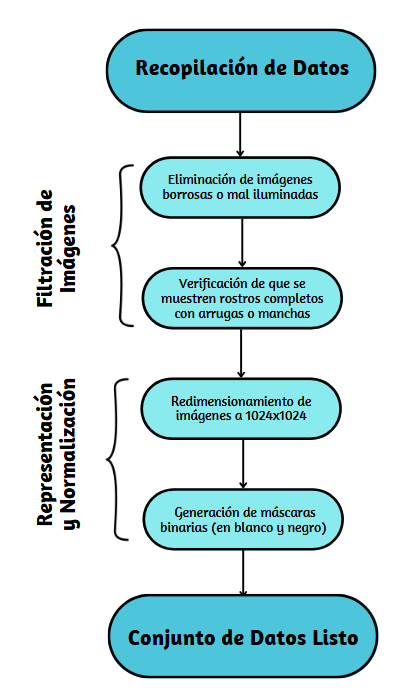
\includegraphics[width=0.45\textwidth]{4/figures/diagrama final prepo.png}
		\caption[Diagrama de Preprocesamiento Utilizado]{Diagrama de Preprocesamiento Utilizado.\\
		Fuente: Elaboración propia}
		\label{4:fig2}
	\end{center}
\end{figure}

\section{Desarrollo de los Modelos de Segmentación}

\subsection{Modelo de Segmentación: Unet}

\subsection{Modelo de Segmentación: UNetAttention}

\subsubsection{Diseño de la arquitectura del modelo}


La arquitectura propuesta se basa en el modelo \textbf{U-Net con mecanismos de atención} (\texttt{UNetAttention}), que combina una red convolucional simétrica tipo encoder-decoder con puertas de atención (\texttt{AttentionGate}) para mejorar el enfoque en las regiones relevantes de la imagen.

\textbf{Encoder (Codificador)}
El encoder está diseñado para capturar características de bajo a alto nivel a partir de la imagen de entrada. Consiste en cuatro bloques llamados \texttt{DoubleConv}:
\begin{itemize}
    \item \textbf{Encoder 1}: Dos convoluciones $3\times3$ (con \texttt{padding}=1), normalización por lotes (BatchNorm) y activación ReLU. Extrae características básicas (bordes, texturas) de las entradas con 3 canales (RGB) y produce 64 mapas de características.
    \item \textbf{Encoder 2}: Similar al anterior, pero recibe 64 mapas y genera 128, aumentando la capacidad de representación.
    \item \textbf{Encoder 3}: Pasa de 128 a 256 mapas, detectando patrones más complejos.
    \item \textbf{Encoder 4}: Pasa de 256 a 512 mapas, capturando características globales.
\end{itemize}
Cada bloque está seguido de una capa \texttt{MaxPool2d(2)}, que reduce la resolución a la mitad e incrementa el campo receptivo, permitiendo captar relaciones espaciales más amplias.

\textbf{Puente (Bottleneck)}
Entre el encoder y el decoder se encuentra el \textbf{bottleneck}, otra capa \texttt{DoubleConv} que recibe 512 mapas y genera 1024. Esta parte actúa como un resumen altamente condensado de toda la información, crucial para sintetizar las representaciones aprendidas antes de reconstruirlas.

\textbf{Attention Gates (Puertas de Atención)}
En lugar de pasar directamente los mapas del encoder al decoder (skip connections), se introducen mecanismos de atención:
\begin{itemize}
    \item Cada \texttt{AttentionGate} recibe dos entradas: $g$ (señal del decoder) y $x$ (señal del encoder).
    \item Ambas se alinean en dimensiones espaciales y se transforman con convoluciones $1\times1$ para reducir canales.
    \item La suma de ambas se activa con ReLU, pasa por otra convolución $1\times1$, BatchNorm y una función sigmoide, generando un mapa de atención $\psi$ entre 0 y 1.
    \item Finalmente, $\psi$ se multiplica por la señal $x$ para filtrar solo las características relevantes.
\end{itemize}
Esto asegura que solo la información útil del encoder fluya al decoder, reduciendo el ruido y enfocándose en las regiones clave.

\textbf{Decoder (Decodificador)}
El decoder reconstruye la imagen segmentada paso a paso:
\begin{itemize}
    \item \textbf{Upconv4}: Upsampling (\texttt{ConvTranspose2d}) de 1024 a 512, concatenado con la salida del encoder4 filtrado por la atención (att3).
    \item \textbf{Decoder4}: \texttt{DoubleConv} que procesa los 1024 canales concatenados y produce 512.
    \item \textbf{Upconv3}, \textbf{Decoder3}: De 512 a 256, concatenado con att2, procesado a 256.
    \item \textbf{Upconv2}, \textbf{Decoder2}: De 256 a 128, concatenado con att1, procesado a 128.
    \item \textbf{Upconv1}, \textbf{Decoder1}: De 128 a 64, concatenado con enc1 (sin atención), procesado a 64.
\end{itemize}

\textbf{Capa Final}
La capa final es una convolución $1\times1$ que reduce los 64 mapas de características a un solo canal de salida (\texttt{out\_channels=1}), generando el mapa binario segmentado.

\textbf{Razones del Diseño}
\begin{itemize}
    \item \textbf{Convoluciones dobles}: Mejoran la capacidad de aprendizaje local sin aumentar demasiado la profundidad.
    \item \textbf{BatchNorm}: Acelera la convergencia y estabiliza el entrenamiento.
    \item \textbf{Atención}: Permite que el modelo se enfoque en las regiones importantes, evitando pasar ruido del encoder al decoder.
    \item \textbf{Skip connections}: Ayudan a recuperar detalles espaciales perdidos por el pooling.
    \item \textbf{Puertas de atención}: Añaden un mecanismo de filtrado adaptativo, crucial en tareas donde no toda la información del encoder es igualmente relevante.
    \item \textbf{Upsampling con transposed convolutions}: Permite recuperar resolución espacial de manera más precisa que el simple escalado.
\end{itemize}

\textbf{Detalle del Funcionamiento}
El proceso completo del modelo se detalla de la siguiente manera:
\begin{enumerate}
\item La imagen de entrada se procesa a través del encoder, extrayendo características jerárquicas que van desde bordes simples hasta patrones complejos, reduciendo la resolución pero aumentando la abstracción.
\item El bottleneck actúa como un cuello de botella que condensa toda la información del encoder en una representación compacta y de alto nivel.
\item El decoder empieza a recuperar la resolución original usando operaciones de upsampling, reconstruyendo progresivamente el mapa segmentado.
\item En cada paso del decoder, las características recuperadas se enriquecen mediante la concatenación de información relevante proveniente del encoder, filtrada cuidadosamente por las puertas de atención.
\item Las puertas de atención permiten que el modelo ignore información irrelevante y se enfoque en regiones específicas de interés para la tarea de segmentación.
\item Finalmente, la capa de salida transforma las características finales en una máscara binaria que identifica las regiones segmentadas de interés en la imagen.
\end{enumerate}

Este funcionamiento asegura que el modelo combine detalles locales finos con contexto global y mecanismos de relevancia, logrando una segmentación precisa y robusta.

\textbf{Pseudocódigo del Modelo}
\begin{verbatim}
Input: Imagen X

# Encoder
enc1 = DoubleConv(X)
enc2 = DoubleConv(MaxPool(enc1))
enc3 = DoubleConv(MaxPool(enc2))
enc4 = DoubleConv(MaxPool(enc3))

# Bottleneck
bottleneck = DoubleConv(MaxPool(enc4))

# Decoder con atención
up4 = UpConv(bottleneck)
att3 = AttentionGate(up4, enc4)
up4_cat = Concatenate(up4, att3)
dec4 = DoubleConv(up4_cat)

up3 = UpConv(dec4)
att2 = AttentionGate(up3, enc3)
up3_cat = Concatenate(up3, att2)
dec3 = DoubleConv(up3_cat)

up2 = UpConv(dec3)
att1 = AttentionGate(up2, enc2)
up2_cat = Concatenate(up2, att1)
dec2 = DoubleConv(up2_cat)

up1 = UpConv(dec2)
up1_cat = Concatenate(up1, enc1)
dec1 = DoubleConv(up1_cat)

# Salida final
Output = Conv1x1(dec1)
Return Output
\end{verbatim}

\subsubsection{Definición de componentes del modelo}
En esta actividad se definen los módulos fundamentales y los elementos de entrenamiento que constituyen el modelo UNetAttention. A continuación se describe en detalle cada uno:

\textbf{1. Módulos arquitectónicos}

\begin{itemize}
\item \textbf{DoubleConv}:
Es un bloque formado por dos capas convolucionales secuenciales, cada una seguida de Batch Normalization y activación ReLU.
Este bloque permite:
\begin{itemize}
\item Extraer patrones locales en múltiples niveles.
\item Evitar problemas de saturación o desaparición de gradientes gracias a ReLU.
\item Estabilizar y acelerar el entrenamiento mediante BatchNorm, que normaliza las salidas y reduce la dependencia de la inicialización.
\end{itemize}

\item \textbf{AttentionGate}:
Es un módulo que implementa un mecanismo de atención espacial. Su estructura:
\begin{itemize}
\item Dos entradas: 
$\mathbf{x}$ (del encoder) y $\mathbf{g}$ (del decoder)

g (del decoder).
\item Aplicación de convoluciones 
1
×
1
1×1 para reducir dimensionalidad.
\item Suma de las dos señales transformadas y paso por activación ReLU.
\item Otra convolución 
1
×
1
1×1 seguida de BatchNorm y activación Sigmoid, que genera un mapa de atención 
\item Multiplicación punto a punto de $\psi$ con $\mathbf{x}$, filtrando las características relevantes.

x, filtrando las características relevantes.
\end{itemize}
El objetivo es permitir al modelo “enfocarse” solo en las regiones de interés para la tarea de segmentación, reduciendo ruido y mejorando la precisión espacial.

\item \textbf{UpConv (Transposed Convolution)}:
Operación que realiza upsampling aprendido, permitiendo reconstruir la resolución espacial en el decoder. Es superior al upsampling por interpolación porque también aprende qué características son importantes al expandir.

\item \textbf{Conv1x1 final}:
Capa de convolución 
1
×
1
1×1 que reduce los canales finales a uno solo (para segmentación binaria), generando la máscara final.
\end{itemize}

\textbf{2. Componentes de entrenamiento}
\begin{itemize}
    \item \textbf{Optimizador \texttt{AdamW}}:
    El optimizador \texttt{AdamW} es una variante de \texttt{Adam} que incluye decaimiento de pesos (weight decay) como un término de regularización, lo que ayuda a prevenir el sobreajuste durante el entrenamiento. AdamW es particularmente útil para redes neuronales profundas donde los modelos tienden a tener una gran cantidad de parámetros. A continuación se detallan los elementos clave de \texttt{AdamW}:
    
    \begin{itemize}
        \item \textbf{Tasas de Aprendizaje Adaptativas}: 
        El optimizador AdamW mantiene tasas de aprendizaje adaptativas para cada parámetro, lo que significa que los parámetros que tienen gradientes más grandes recibirán actualizaciones más pequeñas, mientras que los parámetros con gradientes más pequeños recibirán actualizaciones más grandes. Este enfoque permite que el modelo aprenda de manera más eficiente y rápida, sin necesidad de ajustarse manualmente a una tasa de aprendizaje fija para todos los parámetros. 

        \item \textbf{Decaimiento de Pesos Desacoplado}: 
        A diferencia de \texttt{Adam}, donde el decaimiento de pesos (penalización L2) es acoplado a la actualización de los momentos de primer y segundo orden, \texttt{AdamW} desacopla el decaimiento de pesos de la actualización del momento. Esto significa que el decaimiento de pesos se aplica directamente a los parámetros del modelo y no a los momentos, lo que mejora la regularización y permite un mejor control sobre la actualización de los parámetros.

        \item \textbf{Ventajas sobre Adam}: 
        \begin{itemize}
            \item El decaimiento de pesos desacoplado de los momentos mejora la capacidad de generalización del modelo, reduciendo el riesgo de sobreajuste.
            \item El mantenimiento de tasas de aprendizaje adaptativas optimiza la convergencia durante el entrenamiento.
            \item La actualización de parámetros se realiza con base en los gradientes de la función de pérdida, pero también incluye una penalización proporcional al tamaño de los pesos, evitando que crezcan demasiado y afecten negativamente el rendimiento.
        \end{itemize}
        
        La actualización de parámetros en \texttt{AdamW} sigue la siguiente fórmula:
        \[
        \theta_t = \theta_{t-1} - \frac{\eta}{\sqrt{v_t} + \epsilon} m_t - \eta \cdot \lambda \cdot \theta_{t-1}
        \]
        donde:
        \begin{itemize}
            \item \( \theta_t \) es el parámetro actualizado en el paso \( t \),
            \item \( m_t \) es el primer momento (promedio de gradientes),
            \item \( v_t \) es el segundo momento (promedio de los cuadrados de los gradientes),
            \item \( \lambda \) es el factor de decaimiento de pesos (regularización L2),
            \item \( \eta \) es la tasa de aprendizaje.
        \end{itemize}
    \end{itemize}

    \item \textbf{Scheduler \texttt{ReduceLROnPlateau}}:
    El planificador \texttt{ReduceLROnPlateau} ajusta la tasa de aprendizaje durante el entrenamiento en función de una métrica de validación, como la pérdida o precisión de validación. Este planificador reduce la tasa de aprendizaje cuando una métrica deja de mejorar, ayudando a evitar que el optimizador se quede "atascado" en una meseta, lo que puede ocurrir cuando la tasa de aprendizaje es demasiado alta o demasiado baja. A continuación se detallan sus características:
    
    \begin{itemize}
        \item \textbf{Monitoreo de Métrica de Validación}: 
        \texttt{ReduceLROnPlateau} monitoriza una métrica específica de validación, como la pérdida de validación. Cuando esta métrica deja de mejorar durante un número determinado de épocas (\textit{patience}), el planificador reduce la tasa de aprendizaje de manera progresiva.

        \item \textbf{Evitar mesetas en el entrenamiento}: 
        En ocasiones, durante el entrenamiento, el optimizador se puede quedar atrapado en una meseta, donde la métrica de validación se estabiliza y no mejora, aunque el entrenamiento continúe. Reducir la tasa de aprendizaje en estos puntos puede permitir una convergencia más fina y evitar que el modelo se quede estancado en un mínimo local.

        \item \textbf{Convergencia más fina}: 
        A medida que el entrenamiento progresa y el modelo se acerca a una solución óptima, reducir la tasa de aprendizaje permite que el modelo haga ajustes más pequeños pero precisos. Esto es particularmente útil en las etapas finales del entrenamiento, donde la tasa de aprendizaje grande puede causar grandes oscilaciones en los parámetros.

        \item \textbf{Parámetros de Configuración}: 
        Los parámetros clave de \texttt{ReduceLROnPlateau} incluyen:
        \begin{itemize}
            \item \textbf{factor}: Un valor entre 0 y 1 que indica cuánto reducir la tasa de aprendizaje (por ejemplo, 0.1 reducirá la tasa de aprendizaje en un 90\%).
            \item \textbf{patience}: El número de épocas sin mejora antes de que se reduzca la tasa de aprendizaje.
            \item \textbf{min\_lr}: La tasa de aprendizaje mínima que puede alcanzar el optimizador.
        \end{itemize}
    \end{itemize}

    \item \textbf{Función de Pérdida \texttt{CrossEntropyLoss} (con Pesos Balanceados)}:
    La función de pérdida \texttt{CrossEntropyLoss} es adecuada para problemas de clasificación, y se adapta a segmentación de imágenes al tratar cada píxel como una instancia de clasificación. En casos de clases desbalanceadas (como en segmentación de imágenes médicas), se utilizan \textit{pesos balanceados} para abordar este problema. A continuación, se detallan las características de esta función de pérdida:
    
    \begin{itemize}
        \item \textbf{Desbalance de Clases}: 
        En segmentación, es común que las clases estén desbalanceadas, por ejemplo, el fondo puede ocupar la mayor parte de la imagen mientras que las regiones de interés (como una lesión o arruga) son pequeñas. La función \texttt{CrossEntropyLoss} utiliza pesos balanceados para penalizar más fuertemente los errores en las clases minoritarias.
        
        \item \textbf{Cálculo de Pesos Balanceados}:
        Para calcular los pesos de cada clase, se utiliza un enfoque basado en la frecuencia de cada clase en el conjunto de datos. Se emplea el \textit{Median Frequency Balancing}, donde los pesos son calculados en función de la mediana de las frecuencias de aparición de todas las clases en el conjunto de entrenamiento. Este método asegura que las clases menos representadas tengan un mayor peso en la función de pérdida.

        \item \textbf{Impacto en el Entrenamiento}: 
        La asignación de mayores pesos a las clases minoritarias tiene un impacto positivo en la precisión del modelo al hacer que el modelo enfoque su aprendizaje en esas clases más raras. Esto es crucial para la segmentación de regiones pequeñas o poco representadas, como manchas en la piel, lesiones, o áreas específicas de interés en imágenes médicas.

        \item \textbf{Fórmula de la Pérdida}: 
        La fórmula general para la función de pérdida de entropía cruzada con pesos balanceados es:
        \[
        \text{Loss} = - \sum_{i} w_i \cdot y_i \cdot \log(p_i)
        \]
        donde:
        \begin{itemize}
            \item \( y_i \) es la etiqueta verdadera de la clase \( i \),
            \item \( p_i \) es la probabilidad predicha para la clase \( i \),
            \item \( w_i \) es el peso asignado a la clase \( i \) (calculado a partir de la frecuencia).
        \end{itemize}
    \end{itemize}
\end{itemize}

\textbf{3. Resumen de interacción entre componentes}
Durante el entrenamiento:
\begin{enumerate}
\item El modelo recibe imágenes de entrada que son procesadas por los módulos convolucionales y de atención.
\item Las predicciones por píxel son comparadas contra las máscaras reales usando la función de pérdida ponderada.
\item El optimizador AdamW ajusta los pesos del modelo minimizando la pérdida.
\item El scheduler supervisa la evolución de la métrica de validación y adapta la tasa de aprendizaje si es necesario.
\end{enumerate}

Este conjunto de componentes fue seleccionado cuidadosamente para equilibrar capacidad, estabilidad, precisión y generalización.

\subsubsection{Entrenamiento del Modelo}
\textbf{Actividad 1: Configuración del entorno de entrenamiento} \\
Se preparó el entorno de ejecución para garantizar que todos los experimentos fueran reproducibles y consistentes, realizando lo siguiente:
\begin{itemize}
\item Se definieron las rutas de los conjuntos de datos: las carpetas \texttt{face\_images}, \texttt{arrugas} y \texttt{manchas} contenían las imágenes originales y las máscaras de segmentación correspondientes.
\item El tamaño de lote (\emph{batch size}) se fijó en 4, equilibrando el uso eficiente de memoria GPU/CPU y la estabilidad del gradiente durante la retropropagación.
\item Las imágenes de entrada se redimensionaron a 256 $\times$ 256 píxeles para asegurar una entrada uniforme al modelo y reducir el costo computacional.
\item La tasa de aprendizaje inicial se estableció en $1 \times 10^{-4}$, un valor conservador para evitar inestabilidad en las primeras épocas de entrenamiento.
\item Se programaron 50 épocas completas, buscando alcanzar la convergencia del modelo observando las métricas a lo largo del tiempo.
\item Se habilitó el uso del dispositivo CUDA (GPU) cuando estaba disponible, y si no, el entrenamiento se realizaba en CPU.
\item Se fijó una semilla aleatoria global en 42 para garantizar reproducibilidad en todas las operaciones pseudoaleatorias (división de datos, inicialización de pesos, aumentos de datos).
\end{itemize}

\textbf{Actividad 2: Aplicación de técnicas de optimización} \\
Con el objetivo de mejorar la generalización y eficiencia del modelo, se incorporaron varias técnicas de optimización:
\begin{itemize}
\item Se aplicaron aumentos de datos usando la biblioteca \texttt{albumentations}, generando variaciones artificiales en las imágenes para enriquecer el conjunto de entrenamiento y reducir el sobreajuste. Las transformaciones aplicadas fueron:
  \begin{itemize}
  \item \texttt{A.HorizontalFlip(p=0.5)}: aplica volteo horizontal aleatorio con probabilidad 50\%.
  \item \texttt{A.VerticalFlip(p=0.1)}: aplica volteo vertical aleatorio con probabilidad 10\%.
  \item \texttt{A.RandomRotate90(p=0.2)}: rota la imagen aleatoriamente en múltiplos de 90 grados.
  \item \texttt{A.Rotate(limit=15, p=0.3)}: rota la imagen aleatoriamente hasta 15 grados.
  \item \texttt{A.ElasticTransform(alpha=1, sigma=50, approximate=True, p=0.2)}: aplica transformaciones elásticas para simular deformaciones.
  \item \texttt{A.Affine(scale=(0.9, 1.1), translate\_percent=(0.05, 0.05), rotate=(-10, 10), p=0.3)}: realiza escalado, traslación y rotación aleatoria.
  \item \texttt{A.RandomBrightnessContrast(brightness\_limit=0.2, contrast\_limit=0.2, p=0.3)}: modifica aleatoriamente el brillo y contraste.
  \item \texttt{A.GaussNoise(std\_range=(0.2, 0.44), mean\_range=(0, 0), p=0.2)}: añade ruido gaussiano con desviación estándar variable.
  \item \texttt{A.MotionBlur(blur\_limit=3, p=0.1)}: aplica desenfoque de movimiento.
  \item \texttt{A.HueSaturationValue(hue\_shift\_limit=10, sat\_shift\_limit=15, val\_shift\_limit=10, p=0.2)}: ajusta aleatoriamente el tono, la saturación y el valor.
  \item \texttt{A.Resize(256, 256)}: redimensiona la imagen a 256x256 píxeles.
  \item \texttt{ToTensorV2()} : convierte la imagen y máscara en tensores para PyTorch.
  \end{itemize}
  El bloque de código completo utilizado fue:
  \begin{lstlisting}[language=Python]
  train_transforms = A.Compose([
      A.HorizontalFlip(p=0.5),
      A.VerticalFlip(p=0.1),
      A.RandomRotate90(p=0.2),
      A.Rotate(limit=15, p=0.3),
      A.ElasticTransform(alpha=1, sigma=50, approximate=True, p=0.2),
      A.Affine(scale=(0.9, 1.1), translate_percent=(0.05, 0.05), rotate=(-10, 10), p=0.3),
      A.RandomBrightnessContrast(brightness_limit=0.2, contrast_limit=0.2, p=0.3),
      A.GaussNoise(std_range=(0.2, 0.44), mean_range=(0, 0), p=0.2),
      A.MotionBlur(blur_limit=3, p=0.1),
      A.HueSaturationValue(hue_shift_limit=10, sat_shift_limit=15, val_shift_limit=10, p=0.2),
      A.Resize(256, 256),
      ToTensorV2()
  ])
  \end{lstlisting}

\item Para enfrentar el desbalance entre clases (por ejemplo, menor cantidad de píxeles pertenecientes a manchas comparado con piel), se utilizó el enfoque \emph{median frequency balancing}, que asigna pesos inversamente proporcionales a la frecuencia de cada clase. Estos pesos se pasaron como argumento al criterio \texttt{CrossEntropyLoss}, forzando al modelo a prestar más atención a las clases minoritarias.

\item Se eligió el optimizador \texttt{AdamW}, conocido por su manejo eficiente de regularización y su rendimiento robusto en redes convolucionales, junto con un programador de tasa de aprendizaje (\texttt{ReduceLROnPlateau}), que ajustaba dinámicamente la tasa de aprendizaje cuando la métrica de validación (\texttt{val\_loss}) dejaba de mejorar.

\item Se implementó la impresión detallada de métricas al final de cada época, mostrando pérdidas (\texttt{train\_loss}, \texttt{val\_loss}), precisión, coeficiente Dice e índice de Jaccard, lo cual permitió un seguimiento cuantitativo en tiempo real del progreso del modelo.
\end{itemize}




\textbf{Actividad 3: Validación cruzada del rendimiento} \\
Para evaluar la capacidad del modelo de generalizar sobre datos no vistos, se implementó una rutina robusta de validación:
\begin{itemize}
\item Los datos se dividieron en dos subconjuntos, usando un 80\% para entrenamiento y un 20\% para validación, aplicando la función \texttt{train\_test\_split} para asegurar que ambos conjuntos fueran mutuamente exclusivos.
\item Se construyeron \texttt{DataLoaders} separados para el conjunto de entrenamiento y el de validación, permitiendo un procesamiento eficiente por lotes y garantizando que la evaluación se realizara de forma independiente al entrenamiento.
\item En cada época, se recolectaron todas las predicciones del conjunto de validación y se calcularon métricas de segmentación:
  \begin{itemize}
  \item Precisión global de los píxeles predichos.
  \item Coeficiente Dice, que mide la superposición entre las máscaras predichas y las verdaderas.
  \item Índice de Jaccard, que cuantifica la similitud entre los conjuntos predicho y verdadero.
  \end{itemize}
\item Se guardó automáticamente el modelo correspondiente a la menor pérdida de validación obtenida hasta el momento (\emph{early stopping} implícito), almacenando su estado en el archivo \texttt{best\_model\_Unet\_attention\_100\_epochs.pth}. Esto garantizó que, al final del entrenamiento, se contara con el mejor modelo disponible según el criterio de validación.
\end{itemize}

\subsubsection{Evaluación del Modelo}

\textbf{Actividad 1: Preparación de Datos de Validación} \\
Se prepararon cuidadosamente las imágenes de validación aplicando únicamente transformaciones mínimas para asegurar que las métricas reflejaran el rendimiento real del modelo, sin influencias de aumentos artificiales:
\begin{itemize}
  \item \textbf{Redimensionamiento uniforme:} todas las imágenes y máscaras se reescalaron a 256x256 píxeles, asegurando compatibilidad con las dimensiones de entrada del modelo.
  \item \textbf{Conversión a tensores:} las imágenes se transformaron en tensores (\texttt{ToTensorV2}) sin aplicar alteraciones de brillo, contraste, ruido ni geometría, garantizando que las métricas se calcularan sobre datos reales.
  \item \textbf{Construcción de máscara multicategoría:} las máscaras individuales de arrugas y manchas se combinaron en una única máscara de clase múltiple (con valores codificados por categoría), permitiendo al modelo aprender a distinguir ambas clases en un solo paso de inferencia.
\end{itemize}

\vspace{0.5cm}

\textbf{Actividad 2: Definición de Métricas de Evaluación} \\
Para evaluar de manera robusta el desempeño del modelo, se utilizaron las siguientes métricas:
\begin{itemize}
  \item \textbf{Precisión (macro):} mide la proporción de píxeles predichos correctamente entre todas las clases, promediando por igual sin favorecer a clases más grandes.
  \item \textbf{Dice Score (coeficiente de Sørensen-Dice):} calcula el doble de la intersección dividido por la suma de los tamaños predicho y verdadero, reflejando cuánta superposición real se logró en la segmentación.
  \item \textbf{Índice de Jaccard (IoU):} mide la intersección sobre la unión entre predicciones y referencias, siendo una métrica más estricta para evaluar solapamientos exactos.
\end{itemize}

\vspace{0.5cm}

\textbf{Actividad 3: Evaluación del Modelo} \\
El modelo alcanzó los siguientes resultados promedio sobre el conjunto de validación:
\begin{itemize}
  \item \textbf{Pérdida mínima (\texttt{val\_loss}):} 0.0458 (en la época 50).
  \item \textbf{Precisión promedio:} 0.645, indicando que casi dos tercios de los píxeles se clasificaron correctamente.
  \item \textbf{Dice Score promedio:} 0.440, mostrando un nivel medio de superposición entre máscaras predichas y reales.
  \item \textbf{Jaccard Index promedio:} 0.289, reflejando el desafío de obtener coincidencias exactas en regiones complejas.
  \item Se detectaron mejores resultados en la clase \emph{arrugas}, posiblemente por la mayor representación y contraste de textura.
  \item La clase \emph{manchas} presentó métricas ligeramente inferiores, sugiriendo que futuras optimizaciones deberían incluir aumentos más dirigidos a mejorar esta categoría (por ejemplo, resaltando contraste o coloración).
\end{itemize}

\vspace{0.5cm}

Además de los resultados numéricos, se generaron visualizaciones comparativas entre los datos reales y las predicciones del modelo. Estas imágenes permiten evaluar cualitativamente el desempeño del modelo, mostrando tanto los aciertos como las áreas de mejora. A continuación, se presentan tres ejemplos destacados:

\vspace{0.5cm}

\begin{figure}[H]
\centering
\includegraphics[width=0.85\textwidth]{4/figures/comparación9.png}
\caption{Comparación visual: imagen original, máscara real multicategoría y predicción del modelo para un caso con predominio de arrugas.}
\label{fig:validacion1}
\end{figure}

\begin{figure}[H]
\centering
\includegraphics[width=0.85\textwidth]{4/figures/comparación6.png}
\caption{Comparación visual: ejemplo donde se observa el desempeño del modelo en la detección de manchas, destacando regiones correctamente identificadas y algunas áreas faltantes.}
\label{fig:validacion2}
\end{figure}

\begin{figure}[H]
\centering
\includegraphics[width=0.85\textwidth]{4/figures/comparación1.png}
\caption{Comparación visual: caso mixto donde se presentan simultáneamente arrugas y manchas, mostrando la capacidad del modelo para diferenciar ambas clases en un mismo rostro.}
\label{fig:validacion3}
\end{figure}


\section{Despliegue}

\textbf{Actividad 1: Preparación del Entorno de Despliegue}

\textbf{Actividad 2: Despliegue del Modelo en Producción}
